%============================================================
%  Presentación de tesina de grado
%  Sistema SLAM Visual-Inercial Eficiente con Consistencia Global
%  Autor: Tomás Santucci
%  Compilar con: pdflatex presentation.tex  (dos veces)
%============================================================
\documentclass[aspectratio=169,11pt]{beamer}

\usetheme{default}
\usecolortheme{default}
\setbeamertemplate{navigation symbols}{}      % sin símbolos de navegación
\setbeamertemplate{footline}{}                % sin número de slide
\setbeamertemplate{itemize items}[circle]

\usepackage[utf8]{inputenc}
\usepackage[T1]{fontenc}
\usepackage[spanish]{babel}
\usepackage{graphicx}
\usepackage{amsmath,amssymb}
\usepackage{booktabs}
\usepackage{multirow}
\usepackage{multimedia}   % \movie para videos (reproduce en pdfpc / Acrobat)
% Notas del orador embebidas en el PDF para pdfpc.
% `overridenote` hace que los \note{...} de beamer se conviertan en notas de pdfpc.
\usepackage[overridenote]{pdfpc}

\graphicspath{{img/}{img/intro/}{img/method/}{img/experiments/}}

% Imagen encajada en una caja común (normaliza tamaños con distintas relaciones de aspecto)
\newcommand{\boxedimg}[3]{\includegraphics[width=#1,height=#2,keepaspectratio]{#3}}

% Logo centrado verticalmente respecto a los otros de la misma fila
% (cada uno se baja media altura, de modo que su centro quede en la línea base).
\newcommand{\rowlogo}[2]{\raisebox{-0.5\height}{\includegraphics[height=#1]{#2}}}

% Item con "spotlight": normal en la diapositiva 1 (todos visibles),
% resaltado en azul (color del tema) en la diapositiva #1, atenuado en las demás.
\newcommand{\focusitem}[2]{\alt<1,#1>{\alt<#1>{\structure{#2}}{#2}}{\textcolor{gray!55}{#2}}}

% Placeholder grande (reemplazar por la imagen real)
\newcommand{\phbox}[1]{\fbox{\parbox[c][5.5cm][c]{0.85\linewidth}{\centering \textit{Placeholder}\\[0.4em] #1}}}

% Excluir las diapositivas de backup del total de páginas.
% \backupbegin guarda el nº de frame actual; \backupend lo restaura, de modo que
% las diapositivas posteriores no aumentan \inserttotalframenumber (el total mostrado).
\newcounter{finalframe}
\newcommand{\backupbegin}{\setcounter{finalframe}{\value{framenumber}}}
\newcommand{\backupend}{\setcounter{framenumber}{\value{finalframe}}}

% Al comenzar cada sección, mostrar el índice resaltando la sección actual
\AtBeginSection[]{
  \begin{frame}{Contenido}
    \tableofcontents[currentsection]
  \end{frame}
}

%------------------------------------------------------------
\title[VI-SLAM Eficiente con Consistencia Global]{Sistema SLAM Visual-Inercial Eficiente\\con Consistencia Global}
\author[Tomás Santucci]{Tomás Santucci}
\institute[UNR]{Tesina de Grado de la Licenciatura en Ciencias de la Computación\\
Director: Taihú Pire \quad Co-Director: Mateo de Mayo\\
Universidad Nacional de Rosario}
\date{\today}

%============================================================
\begin{document}

%---------------- Portada ----------------
\begin{frame}[plain]
  \titlepage
  \begin{center}
  \rowlogo{1.05cm}{cifasis-logo.pdf}\hspace{2em}%
  \rowlogo{0.85cm}{tum-logo.png}
  \end{center}
  \vspace{0.7cm}
\end{frame}

%---------------- Índice ----------------
\begin{frame}{Contenido}
  \tableofcontents
\end{frame}

%============================================================
\section{Introducción}
%============================================================

\begin{frame}{SLAM}
  \emph{Simultaneous Localization and Mapping}
  \vspace{0.6em}
  \begin{itemize}
    \item Resuelve de manera \textbf{simultánea}:
    \begin{itemize}
      \item la \textbf{localización} de un robot (su pose), y
      \item el \textbf{mapeo} del entorno.
    \end{itemize}
    \item A partir de la información de sus \textbf{sensores}.
    \item Cuando se usan \textbf{cámaras} e \textbf{IMU}, hablamos de \textbf{VI-SLAM} (Visual-Inercial).
  \end{itemize}
\end{frame}

\begin{frame}{Aplicaciones del SLAM}
  \centering
  % Cada imagen se centra dentro de una caja de altura fija para alinear los epígrafes.
  \begin{columns}[t]
    \begin{column}{0.32\textwidth}
      \centering
      \parbox[c][4.2cm][c]{\linewidth}{\centering\boxedimg{\linewidth}{4.2cm}{metaquest3.png}}\\[0.4em]
      {\scriptsize Realidad virtual / aumentada (XR)}
    \end{column}
    \begin{column}{0.32\textwidth}
      \centering
      \parbox[c][4.2cm][c]{\linewidth}{\centering\boxedimg{\linewidth}{4.2cm}{crazyflie.png}}\\[0.4em]
      {\scriptsize Drones}
    \end{column}
    \begin{column}{0.32\textwidth}
      \centering
      \parbox[c][4.2cm][c]{\linewidth}{\centering\boxedimg{\linewidth}{4.2cm}{unweed_robot_re.png}}\\[0.4em]
      {\scriptsize Robótica autónoma}
    \end{column}
  \end{columns}
\end{frame}

\begin{frame}{Desafíos}
  \begin{itemize}
    \item Robustez ante condiciones de XR. % movimientos bruscos, oclusiones, blur
    \item Bajos requisitos computacionales. % la tendencia de los últimos sistemas de SLAM es usar redes neuronales, pero los vuelve más costosos
%    \item Precisión. % mareos en XR
    \item Eficiencia (tiempo real).
  \end{itemize}
  \note{Por que desarrollar otro sistema de SLAM? Ninguno satisface las 3 condiciones simlutaneamente.}
\end{frame}

\begin{frame}{Componentes de un sistema VI-SLAM}
  \begin{columns}[c]
    \begin{column}{0.4\textwidth}
      \large
      \begin{itemize}
        \item \focusitem{2}{Front-end}
        \item \focusitem{3}{Back-end (Basado en grafos)}
        \item \focusitem{4}{Cierre de ciclos}
      \end{itemize}
    \end{column}
    \begin{column}{0.6\textwidth}
      \centering
      % Diapositiva 1: solo los items. Desde la 2, la imagen/video de cada componente.
      % El video se reproduce al hacer clic (pdfpc o Adobe Acrobat); en otros
      % visores se ve el frame poster. El .webm debe quedar junto al PDF.
      \only<2>{\movie[showcontrols,loop]{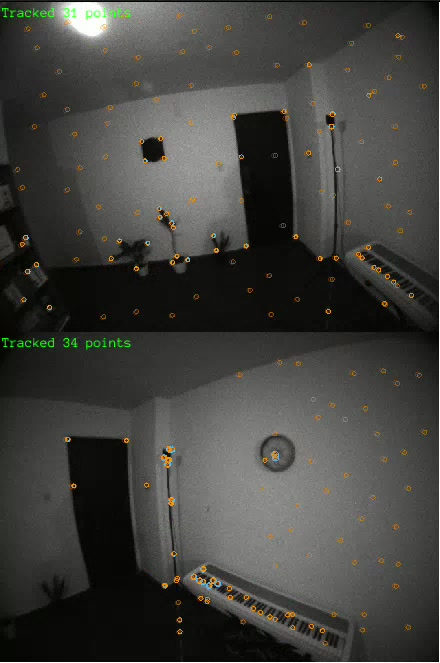
\includegraphics[height=8cm]{videos/front-end.poster.jpg}}{videos/front-end.webm}}%
      \only<3>{%
        \boxedimg{\linewidth}{4.8cm}{factor-graph.pdf}\\[0.9em]
        {\footnotesize $\displaystyle
          E = \sum_{\substack{i \in L \\ t \in \text{obs}(i)}} r_{it}^\top \Sigma_{it}^{-1} r_{it}
            + \sum_{(i,j) \in C} r_{ij}^\top \Sigma_{ij}^{-1} r_{ij} + E_m$}\\[0.6em]
        {\scriptsize reproyección de landmarks + IMU + prior de marginalización.}%
      }%
      \only<4>{\boxedimg{\linewidth}{6cm}{loop-closure.png}}%
    \end{column}
  \end{columns}
\end{frame}

%============================================================
\section{Método}
%============================================================

\begin{frame}{Punto de partida: BasaltMSD}
  \begin{itemize}
    \item \textbf{BasaltMSD} es una extensión de Basalt con:
    \begin{itemize}
      \item Soporte para cámaras no paralelas y $>2$ cámaras.
      \item IMU en el front-end.
      \item \emph{Recall} de features perdidos.
      \item Mapa persistente.
      \item etc.
    \end{itemize}
    \item Arquitectura \textbf{asíncrona}: front-end $\parallel$ back-end (VIO $\parallel$ mapa).
  \end{itemize}
  \note{mencionar tesina de bruno}
  \note{basalt: sistema VIO del estado del arte, tiempo real, preciso y robusto. Con mapper offline}
\end{frame}

\begin{frame}{Arquitectura de BasaltMSD}
  \centering
  \boxedimg{\linewidth}{0.82\textheight}{arch.basaltmsd.pdf}
\end{frame}

\begin{frame}{Aportes de este trabajo}
  Sobre BasaltMSD se incorporan, respetando su arquitectura asíncrona:
  \vspace{0.4em}
  \begin{enumerate}
    \item<1-> Cierre de ciclos en tiempo real.
    \item<2-> Eliminación de keyframes.
    \item<3-> Bundle Adjustment global con RootBA.
  \end{enumerate}
\end{frame}

\begin{frame}{Nueva arquitectura}
  \centering
  \boxedimg{\linewidth}{0.82\textheight}{arch.full.pdf}
\end{frame}

\begin{frame}[t]{1- Cierre de ciclos: detección}
  \centering
  \boxedimg{\linewidth}{0.2\textheight}{loop-closure-1.png}%
  \only<2>{\\[5em]
    \boxedimg{\linewidth}{0.6\textheight}{bow-process.pdf}%
  }
  \only<3->{\\[1em]
    \boxedimg{\linewidth}{0.6\textheight}{hashbow.pdf}%
  }
\end{frame}

\begin{frame}[t]{1- Cierre de ciclos: verificación}
  \centering
  \boxedimg{\linewidth}{0.2\textheight}{loop-closure-2.png}%
  \only<2->{\\[1em]
    \boxedimg{\linewidth}{0.6\textheight}{island-sp.pdf}%
  }
\end{frame}

\begin{frame}[t]{1- Cierre de ciclos: optimización}
  \centering
  \boxedimg{\linewidth}{0.2\textheight}{loop-closure-3.png}\\[3em]
  \begin{columns}[c]
    \begin{column}{0.58\textwidth}
      \centering
      \only<2>{\boxedimg{\linewidth}{0.38\textheight}{pose-graph-1.pdf}}%
      \only<3>{\boxedimg{\linewidth}{0.38\textheight}{pose-graph-2.pdf}}%
      \only<4->{\boxedimg{\linewidth}{0.38\textheight}{pose-graph-3.pdf}}%
    \end{column}
    \begin{column}{0.42\textwidth}
      \centering
      \only<5->{$\displaystyle
        E = \sum_{(i, j)} \left\|\log\!\left(\tilde{\mathbf{T}}_{ij}^{-1}\mathbf{T}_{ij}\right)^\vee\right\|^2$}%
    \end{column}
  \end{columns}
\end{frame}

\begin{frame}{2- Eliminación de keyframes}
  \begin{columns}[c]
    \begin{column}{0.56\textwidth}
      \begin{itemize}
        \item Redundancia.
        \item Límite de tamaño. Basado en un puntaje:
        \[ \text{score} = 0.4\,S_g + 0.2\,S_l + 0.2\,S_o + 0.1\,S_c + 0.1\,S_t \]
      \end{itemize}
    \end{column}
    \begin{column}{0.44\textwidth}
      \centering
      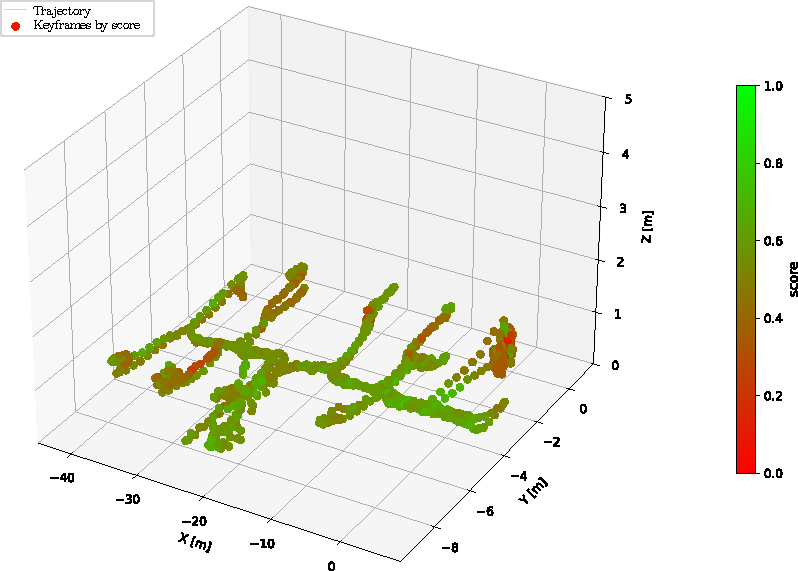
\includegraphics[width=\textwidth]{culling-scores.pdf}\\
      {\scriptsize Puntajes de keyframes del mapa.}
    \end{column}
  \end{columns}
  \note{Sg: reemplazabilidad en el grafo. Sl: participacion en loops. So: cantidad de observaciones. Sc: cubrimiento de imagen. St: posicion temporal.}
\end{frame}

\begin{frame}{3- RootBA: introducción}
  \begin{columns}[c]
    \begin{column}{0.5\textwidth}
      \centering
      \boxedimg{\linewidth}{0.78\textheight}{ba.png}\\[0.2em]
      {\scriptsize Bundle adjustment en Structure from Motion.}
    \end{column}
    \begin{column}{0.5\textwidth}
      Minimiza el \textbf{error de reproyección} acumulado sobre todas las observaciones:
      \[ E(x_p, x_l) = \sum_{i}\ \sum_{j \in \mathcal{O}(i)} \left\| r_{ij}(x_p, x_l) \right\|^2 \]
      {\footnotesize
      \begin{itemize}
        \item $x_p$: poses de las cámaras; $x_l$: landmarks.
        \item $j \in \mathcal{O}(i)$: el landmark $j$ se observa en el frame $i$.
        \item $r_{ij}$: residual de reproyección.
      \end{itemize}}
    \end{column}
  \end{columns}
\end{frame}

\begin{frame}{3- RootBA: en optimización global de SLAM}
  \begin{columns}[c]
    \begin{column}{0.55\textwidth}
      \begin{itemize}
        \item<2-> No optimiza los parámetros intrínsecos de las cámaras.
        \item<3-> Reparametriza el estado para soportar sistemas multi-cámara.
        \item<4-> Soporte para modelos de cámaras arbitrarios.
        \item<5-> Nuevo estado: $s=(s_b, s_l)$.
      \end{itemize}
    \end{column}
    \begin{column}{0.45\textwidth}
      \centering
      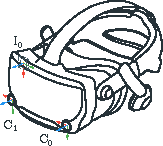
\includegraphics[width=\textwidth]{rig.pdf}\\
      {\scriptsize Ejemplo de un sistema multi-cámara.}
    \end{column}
  \end{columns}
  \note{asumimos que las cámaras no se mueven y también que los intrínsecos no cambian}
\end{frame}

\begin{frame}[t]{3- RootBA: adaptaciones detalle}
  \begin{figure}[!htbp]
      \centering
      
\includegraphics[width=0.8\linewidth]{img/method/rootba-mod.pdf}
      \caption{Estructura de un Landmark Block.}
      \label{fig:landmark_block}
  \end{figure}

  \only<2->{%
  Aplicando la regla de la cadena, el jacobiano del residual respecto a $x_b$ queda:
  \begin{equation}
  \frac{\partial r}{\partial \Delta x_b} = \frac{\partial r}{\partial \Delta x_{c_k}} \cdot \frac{\partial \Delta x_{c_k}}{\partial \Delta x_b} = \frac{\partial r}{\partial \Delta x_{c_k}}\cdot \mathrm{Ad}_{T_{c_k b}}.
  \end{equation}%
  }
\end{frame}

%============================================================
\section{Experimentos}
%============================================================

% TODO: simplificar en 1 sola slide
%\begin{frame}{Datasets (poner videos)}
%  \begin{columns}[c]
%    \begin{column}{0.38\textwidth}
%      \large
%      \begin{itemize}
%        \item \focusitem{2}{EuRoC {\footnotesize(dron, interiores)}}
%        \item \focusitem{3}{TUM-VI {\footnotesize(\emph{handheld})}}
%        \item \focusitem{4}{MSD {\footnotesize(XR, \textit{headsets})}}
%      \end{itemize}
%      \vspace{0.6em}
%      {\footnotesize Cubren baja textura, movimientos rápidos y trayectorias largas.}
%    \end{column}
%    \begin{column}{0.62\textwidth}
%      \centering
%      % Diapositiva 1: solo los items. Desde la 2: frame de la secuencia + dispositivo(s).
%      \only<2>{%
%        \boxedimg{\linewidth}{3cm}{MH03.jpg}\\[0.15em]
%        {\scriptsize Secuencia (Machine Hall)}\\[0.7em]
%        \boxedimg{0.5\linewidth}{2.8cm}{euroc-device.jpg}\\[0.15em]
%        {\scriptsize Dispositivo: micro-dron (MAV)}%
%      }%
%      \only<3>{%
%        \boxedimg{\linewidth}{3cm}{TR4.jpg}\\[0.15em]
%        {\scriptsize Secuencia (\emph{room})}\\[0.7em]
%        \boxedimg{0.5\linewidth}{2.8cm}{tumvi-device.jpg}\\[0.15em]
%        {\scriptsize Dispositivo: cámara \emph{handheld}}%
%      }%
%      \only<4>{%
%        \boxedimg{\linewidth}{3cm}{MIPT02.1.jpg}\\[0.15em]
%        {\scriptsize Secuencia (hasta 40 min)}\\[0.6em]
%        \boxedimg{0.31\linewidth}{2cm}{headset.VI.png}\hfill
%        \boxedimg{0.31\linewidth}{2cm}{headset.OPlus.png}\hfill
%        \boxedimg{0.31\linewidth}{2cm}{headset.RG2V2.png}\\[0.15em]
%        {\scriptsize Cascos: Valve Index, Odyssey+, Reverb G2 V2}%
%      }%
%    \end{column}
%  \end{columns}
%\end{frame}

% Versión resumida en una sola diapositiva (sin overlays) de la anterior.
\begin{frame}{Datasets}
  \centering
  % Cajas de altura fija para que las tres columnas queden alineadas.
  \begin{columns}[t]
    \begin{column}{0.32\textwidth}
      \centering
      \textbf{EuRoC}\\[0.4em]
      \parbox[c][3cm][c]{\linewidth}{\centering\boxedimg{\linewidth}{3cm}{MH03.jpg}}\\[0.5em]
      \parbox[c][1.8cm][c]{\linewidth}{\centering\boxedimg{\linewidth}{1.8cm}{euroc-device.jpg}}\\[0.3em]
      {\scriptsize Micro-dron (MAV), interiores}
    \end{column}
    \begin{column}{0.32\textwidth}
      \centering
      \textbf{TUM-VI}\\[0.4em]
      \parbox[c][3cm][c]{\linewidth}{\centering\boxedimg{\linewidth}{3cm}{TR4.jpg}}\\[0.5em]
      \parbox[c][1.8cm][c]{\linewidth}{\centering\boxedimg{\linewidth}{1.8cm}{tumvi-device.jpg}}\\[0.3em]
      {\scriptsize Cámara \emph{handheld}, interiores y exteriores}
    \end{column}
    \begin{column}{0.32\textwidth}
      \centering
      \textbf{MSD}\\[0.4em]
      \parbox[c][3cm][c]{\linewidth}{\centering\boxedimg{\linewidth}{3cm}{MIPT02.1.jpg}}\\[0.5em]
      \parbox[c][1.8cm][c]{\linewidth}{\centering%
        \boxedimg{0.9\linewidth}{1.8cm}{devices.pdf}}\\[0.3em]
%        \boxedimg{0.3\linewidth}{1.8cm}{headset.VI.png}\hfill
%        \boxedimg{0.3\linewidth}{1.8cm}{headset.OPlus.png}\hfill
%        \boxedimg{0.3\linewidth}{1.8cm}{headset.RG2V2.png}}\\[0.3em]
      {\scriptsize Cascos XR (Valve Index, Odyssey+, Reverb G2 V2), hasta 40 min}
    \end{column}
  \end{columns}
  \vspace{0.8em}
  {\footnotesize Cubren baja textura, movimientos rápidos y trayectorias largas.}
\end{frame}

\begin{frame}{Estudio de ablación}
  Se incorporan las mejoras progresivamente:
  \begin{itemize}
    \item \textbf{BasaltMSD}: sistema original (VIO).
    \item \textbf{BasaltLC}: mapa persistente, loop closure y culling.
    \item \textbf{BasaltLCR}: optimización global con RootBA.
  \end{itemize}
\end{frame}

\begin{frame}{BasaltLC - GUI}
  \centering
  \movie[showcontrols,loop]{\boxedimg{\linewidth}{0.88\textheight}{videos/MPX.poster.jpg}}{videos/MPX.webm}
\end{frame}

\begin{frame}{Mapas obtenidos por BasaltMSD, BasaltLC y BasaltLCR}
  \centering
  \begin{columns}[t]
    \begin{column}{0.33\textwidth}
      \centering
      \boxedimg{\linewidth}{0.72\textheight}{MGO01.vio.map.png}\\[0.3em]
      {\scriptsize BasaltMSD (VIO)}
    \end{column}
    \begin{column}{0.33\textwidth}
      \centering
      \boxedimg{\linewidth}{0.72\textheight}{MGO01.lc.map.png}\\[0.3em]
      {\scriptsize BasaltLC (+ loop closure)}
    \end{column}
    \begin{column}{0.33\textwidth}
      \centering
      \boxedimg{\linewidth}{0.72\textheight}{MGO01.full.map.png}\\[0.3em]
      {\scriptsize BasaltLCR (+ BA global)}
    \end{column}
  \end{columns}
\end{frame}

\begin{frame}{Sistema propuesto vs. estado del arte en EuRoC y TUM-VI}
  \begin{table}[!htbp]
  \centering
  \caption{Resumen de la comparación con el estado del arte: ATE [m] promedio por grupo de secuencias en los datasets EuRoC y TUM-VI.}
  \label{tab:sota_summary_ate}
  \begin{tabular}{ll rrrr}
  \toprule
  \textbf{Dataset} & \textbf{Grupo} & \textbf{BasaltMSD} & \textbf{BasaltLCR} & \textbf{OKVIS2} & \textbf{ORB-SLAM3} \\
  \midrule
  \multirow{5}{*}{TUM-VI}
  & Corridor    & 0.39 & 0.08 & 0.09 & \textbf{0.06} \\
  & Magistrale  & 1.84 & 0.85 & \textbf{0.28} & 0.81 \\
  & Outdoors    & 60.19 & 62.26 & \textbf{11.60} & 17.87 \\
  & Room        & 0.09 & \textbf{0.01} & \textbf{0.01} & \textbf{0.01} \\
  & Slides      & 1.03 & 0.92 & 0.54 & \textbf{0.46} \\
  \midrule
  \multirow{3}{*}{EuRoC}
  & Machine Hall  & 0.09 & 0.08 & \textbf{0.04} & 0.05 \\
  & Vicon Room 1  & 0.05 & 0.07 & \textbf{0.02} & 0.03 \\
  & Vicon Room 2  & 0.08 & 0.09 & \textbf{0.02} & \textbf{0.02} \\
  \bottomrule
  \end{tabular}
  \end{table}
\end{frame}

\begin{frame}{Sistema propuesto vs. estado del arte en MSD}
  \begin{table}[!htbp]
  \centering
  \caption{Resumen de la comparación con el estado del arte: ATE [cm], RTE [cm] y tasa de completitud (\%) promedio por headset en MSD.}
  \label{tab:msd_sota_summary}
  \resizebox{\textwidth}{!}{
  \begin{tabular}{l rrrr | rrrr | rrrr}
  \toprule
  & \multicolumn{4}{c|}{\textbf{ATE [cm]}} & \multicolumn{4}{c|}{\textbf{RTE [cm]}} & \multicolumn{4}{c}{\textbf{Completitud (\%)}} \\
  \cmidrule(lr){2-5} \cmidrule(lr){6-9} \cmidrule(lr){10-13}
  \textbf{Headset}
  & \rotatebox{90}{\textbf{BasaltMSD}\,}
  & \rotatebox{90}{\textbf{BasaltLCR}\,}
  & \rotatebox{90}{\textbf{OKVIS2}\,}
  & \rotatebox{90}{\textbf{ORB-SLAM3}\,}
  & \rotatebox{90}{\textbf{BasaltMSD}\,}
  & \rotatebox{90}{\textbf{BasaltLCR}\,}
  & \rotatebox{90}{\textbf{OKVIS2}\,}
  & \rotatebox{90}{\textbf{ORB-SLAM3}\,}
  & \rotatebox{90}{\textbf{BasaltMSD}\,}
  & \rotatebox{90}{\textbf{BasaltLCR}\,}
  & \rotatebox{90}{\textbf{OKVIS2}\,}
  & \rotatebox{90}{\textbf{ORB-SLAM3}\,} \\
  \midrule
  Valve Index (MI*)      & 28.0 & \textbf{5.4} & 220.4 & 17309.9 & \textbf{1.0} & 1.4 & 3.1 & 80.7 & \textbf{100} & \textbf{100} & \textbf{100} & 91 \\
  HP Reverb G2 (MG*)     & 21.7 & \textbf{4.0} & 10.5 & 827.1 & 1.4 & 1.6 & \textbf{0.9} & 11.5 & \textbf{100} & \textbf{100} & \textbf{100} & 98 \\
  Samsung Odyssey+ (MO*) & 26.7 & \textbf{21.3} & 42.9 & 21.7 & 1.1 & 1.8 & \textbf{0.8} & 7.9 & \textbf{100} & \textbf{100} & \textbf{100} & 92 \\
  \bottomrule
  \end{tabular}
  }
  \end{table}
\end{frame}

\begin{frame}{Sistema propuesto vs. estado del arte: Timings}
  \centering
  \boxedimg{\linewidth}{0.82\textheight}{MGO04.timings-sp.pdf}
\end{frame}

\begin{frame}{RootBA: precisión simple vs. doble}
  \centering
  \boxedimg{\linewidth}{0.82\textheight}{msd.rootba.times-sp.pdf}
\end{frame}

%============================================================
\section{Conclusión}
%============================================================

\begin{frame}{Conclusiones: aportes}
  \begin{itemize}
    \item VI-SLAM eficiente sobre BasaltMSD: \textbf{cierre de ciclos, eliminación de keyframes y Bundle Adjustment global}, bajo arquitectura asíncrona (sin degradar el rendimiento).
    \item Detección de ciclos con \textbf{HashBoW} y cadena de verificaciones robustas.
    \item \textbf{Primera aplicación de RootBA} como BA global en VI-SLAM: multicámara y precisión simple ($-50\%$ de tiempo).
    \item Mejor combinación de \textbf{precisión, robustez y tiempo real} en XR; supera a ORB-SLAM3 y OKVIS2.
    \item Se envió el trabajo a las Jornadas Argentinas de Robótica (JAR) 2026.
    \item Se utilizó el cierre de ciclos en un trabajo de Mattis Krauch para el Hilti x Trimble SLAM Challenge 2026, quedando \#9.
    \note{Se esta usando en un sisteme de Gaussian Splatting en real-time}
  \end{itemize}
\end{frame}

\begin{frame}{Trabajo futuro}
  \begin{itemize}
    \item BA online, integrado al mapa persistente.
    \item Términos de IMU / pose relativa en la optimización global.
    \item Verificación de ciclos más robusta (entornos difíciles).
    \item Colaboración multiagente sobre un mapa compartido.
    \note{La intencion es publicar en ICRA}
  \end{itemize}
\end{frame}

\begin{frame}[plain]
  \vfill
  \begin{center}
    {\Huge \textbf{¡Gracias!}}\\[2.5em]
    \begin{tabular}{r@{\hspace{1.5em}}l}
      \textbf{Tomás Santucci}        & \texttt{tomassantucci0@gmail.com} \\[0.6em]
      \textbf{Taihú Pire}            & \texttt{pire@cifasis-conicet.gov.ar} \\[0.2em]
      {\footnotesize Director}       & \\[0.6em]
      \textbf{Mateo de Mayo}         & \texttt{mateo.demayo@tum.de} \\[0.2em]
      {\footnotesize Co-Director}    & \\
    \end{tabular}
  \end{center}
  \vfill
\end{frame}

%---------------- Backup: no cuenta para el total de páginas ----------------
\backupbegin

\begin{frame}{Fusión de mapa}
  Etapa final del proceso, se ejecute o no PGO. Comprende tres pasos:
  \vspace{0.5em}
  \begin{enumerate}
    \item \textbf{Aplicar} las poses optimizadas al mapa (incorporando keyframes llegados durante la optimización).
    \item \textbf{Registrar} el ciclo en el grafo de ciclos (arista $k_r \leftrightarrow k_c$).
    \item \textbf{Fusionar} landmarks duplicados: un mismo punto del mundo con dos identificadores distintos se unifica, transfiriendo todas sus observaciones.
  \end{enumerate}
  \vspace{0.5em}
  \begin{itemize}
    \item Tras cada modificación se actualiza el grafo de covisibilidad ponderado para mantener el mapa consistente.
  \end{itemize}
\end{frame}

\begin{frame}{Métricas y tiempo real}
  \begin{itemize}
    \item \textbf{ATE} (Absolute Trajectory Error): precisión global de la trayectoria.
    \item \textbf{RTE} (Relative Trajectory Error): consistencia local.
    \item Evaluación \textbf{no causal} (trayectoria final, con correcciones aplicadas).
  \end{itemize}
  \vspace{0.4em}
  \begin{block}{Límites de tiempo real (ms por frame)}
    \centering
    Valve Index: \textbf{18.5} \quad | \quad Odyssey+ / Reverb G2: \textbf{33.3} \quad | \quad EuRoC / TUM-VI: \textbf{50}
  \end{block}
  \begin{itemize}
    \item Tres modos de ejecución: síncrono, \textbf{asíncrono}, y síncrono con mapa asíncrono.
  \end{itemize}
\end{frame}

\begin{frame}{Rendimiento: trayectorias extensas y tiempo real (cambiarlo por el gráfico de PGO)}
  \begin{columns}[c]
    \begin{column}{0.5\textwidth}
      \centering
      
\includegraphics[width=\textwidth]{kftimings.MGO12-sp.pdf}\\
      {\scriptsize El \textbf{culling} mantiene estable el tiempo por frame en trayectorias $>40$ min; sin él, el costo de PGO crece indefinidamente.}
    \end{column}
    \begin{column}{0.5\textwidth}
      \centering
      
\includegraphics[width=\textwidth]{mean.timings.barplot-sp.pdf}\\
      {\scriptsize La arquitectura asíncrona permite a BasaltLC operar dentro de los límites de tiempo real en todos los headsets, sin degradar el rendimiento base.}
    \end{column}
  \end{columns}
\end{frame}

\begin{frame}{Front-end}
  \begin{columns}[c]
    \begin{column}{0.55\textwidth}
      \begin{itemize}
        \item \textbf{Optical flow} (Lucas-Kanade), con la IMU como \emph{prior} de la posición del keypoint.
        \item \textbf{Recall}: recupera features perdidos por oclusiones o movimientos rápidos, proyectando landmarks del back-end.
        \item Detección \textbf{FAST} por celdas (buena distribución).
        \item \textbf{Matching} multicámara y filtrado por restricción \textbf{epipolar}.
      \end{itemize}
    \end{column}
    \begin{column}{0.45\textwidth}
      \centering
      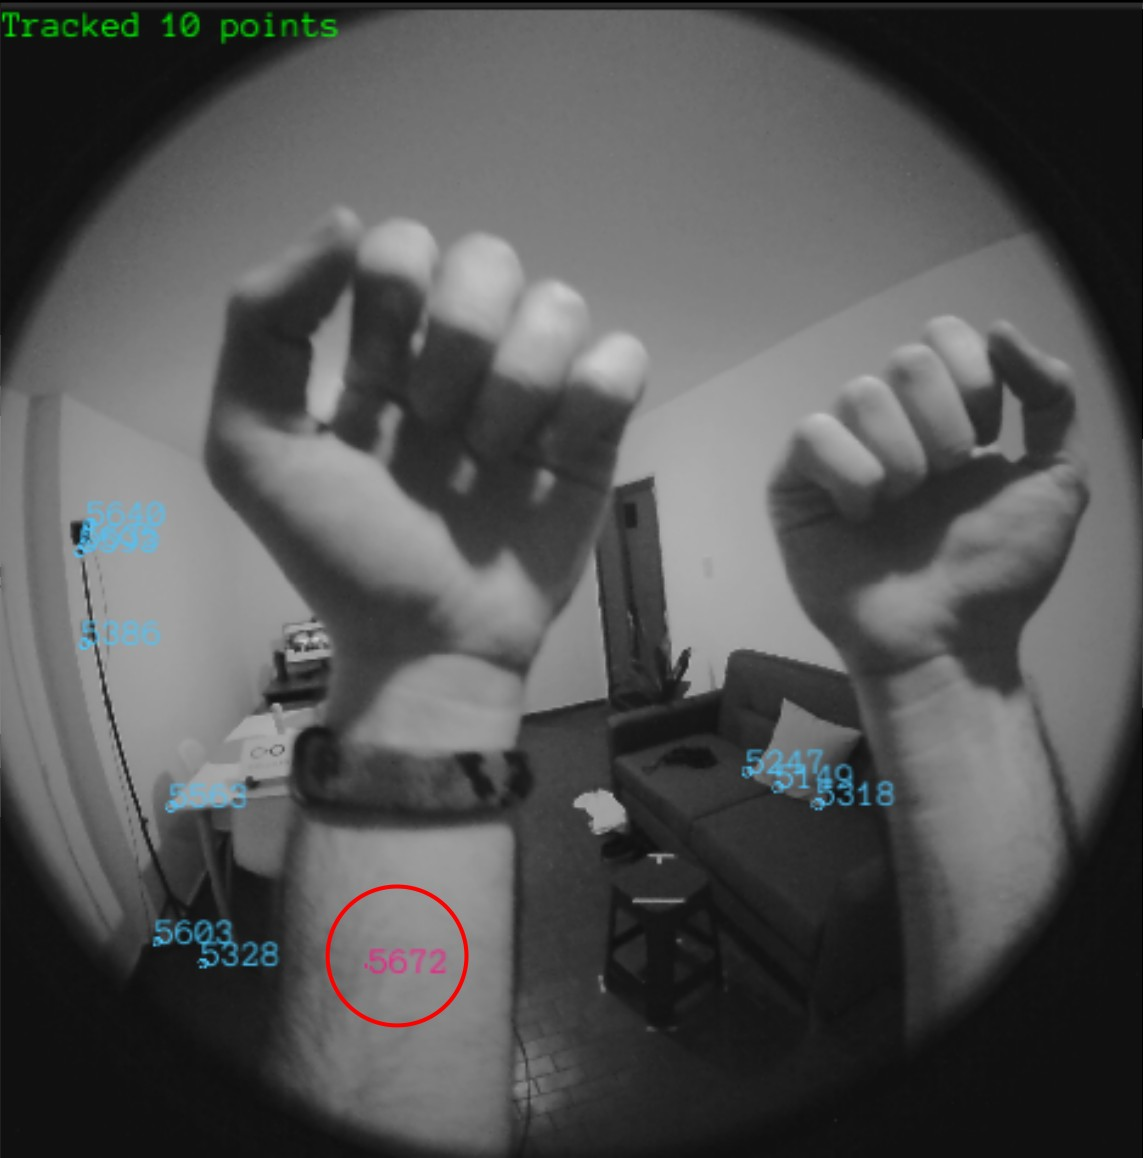
\includegraphics[width=\textwidth]{recall_982.jpg}\\
      {\scriptsize Recall: el feature ocluido se reidentifica proyectando el landmark (en rosa).}
    \end{column}
  \end{columns}
\end{frame}

\begin{frame}{Back-end: VIO}
  \begin{columns}[c]
    \begin{column}{0.55\textwidth}
      \begin{itemize}
        \item Mantiene una \textbf{ventana deslizante} de keyframes, frames y landmarks (\texttt{LandmarkDatabase}).
        \item Preintegra la IMU y optimiza el estado por mínimos cuadrados no lineales (Levenberg-Marquardt):
        \[ E = E_L + E_I + E_m \]
        {\scriptsize reproyección de landmarks + IMU + prior de marginalización.}
        \item \textbf{Marginalización}: elimina variables antiguas condensando su información, para acotar el tamaño del sistema.
      \end{itemize}
    \end{column}
    \begin{column}{0.45\textwidth}
      \centering
      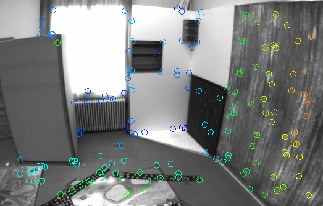
\includegraphics[width=\textwidth]{basalt.vio.window.cam0.pdf}\\
      {\scriptsize Observaciones en la ventana local del VIO.}
    \end{column}
  \end{columns}
\end{frame}

\begin{frame}{Back-end: mapa persistente}
  \begin{columns}[c]
    \begin{column}{0.5\textwidth}
      \begin{itemize}
        \item Almacena keyframes y landmarks a \textbf{largo plazo} $\Rightarrow$ convierte al sistema en \textbf{VI-SLAM}.
        \item Comunicación \textbf{asíncrona} mediante colas: no bloquea al VIO.
        \item \textbf{Consulta de covisibilidad}: reintroduce keyframes ya marginalizados en la ventana local del VIO.
      \end{itemize}
    \end{column}
    \begin{column}{0.5\textwidth}
      \centering
      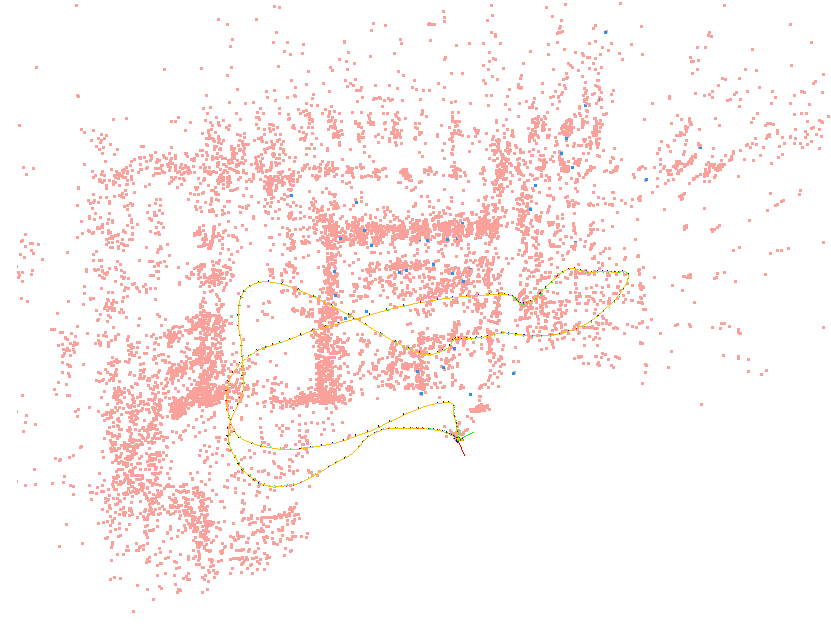
\includegraphics[height=3.2cm]{persistent.map.png}
      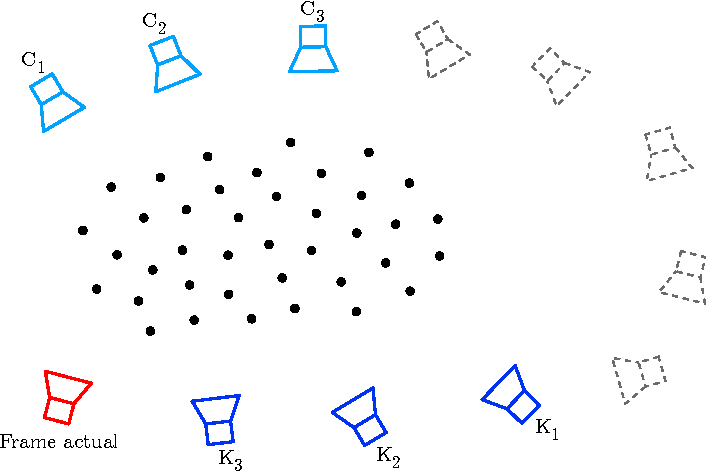
\includegraphics[height=3.2cm]{covisibility-sp.pdf}\\
      {\scriptsize Mapa persistente y reintroducción de keyframes covisibles.}
    \end{column}
  \end{columns}
\end{frame}

\begin{frame}{Ablación: resultados de precisión}
  \centering
  \footnotesize
  \setlength{\tabcolsep}{4.5pt}
  \begin{tabular}{ll rrr | rrr}
  \toprule
  & & \multicolumn{3}{c|}{\textbf{ATE [cm]}} & \multicolumn{3}{c}{\textbf{RTE [cm]}} \\
  \cmidrule(lr){3-5} \cmidrule(lr){6-8}
  \textbf{Dataset} & \textbf{Grupo}
  & \textbf{MSD} & \textbf{LC} & \textbf{LCR}
  & \textbf{MSD} & \textbf{LC} & \textbf{LCR} \\
  \midrule
  \multirow{5}{*}{TUM-VI}
  & Corridor    & 39.2 & 10.9 & \textbf{8.3} & 7.4 & 3.6 & \textbf{2.8} \\
  & Magistrale  & 183.7 & 88.5 & \textbf{84.7} & 22.5 & 10.3 & \textbf{9.6} \\
  & Outdoors    & \textbf{6019.0} & 6227.1 & 6226.1 & \textbf{624.0} & 644.3 & 643.9 \\
  & Room        & 8.7 & 3.7 & \textbf{0.9} & 0.6 & 0.8 & \textbf{0.4} \\
  & Slides      & 102.5 & 92.6 & \textbf{91.8} & 11.8 & 10.9 & \textbf{10.8} \\
  \midrule
  \multirow{3}{*}{EuRoC}
  & Machine Hall  & 9.1 & \textbf{6.8} & 8.2 & \textbf{0.9} & \textbf{0.9} & \textbf{0.9} \\
  & Vicon Room 1  & 5.1 & \textbf{5.0} & 6.7 & \textbf{1.2} & 1.3 & 2.2 \\
  & Vicon Room 2  & 7.8 & \textbf{5.0} & 9.1 & \textbf{1.2} & 1.5 & 3.9 \\
  \midrule
  \multirow{3}{*}{MSD}
  & Valve Index      & 28.0 & 6.6 & \textbf{5.4} & \textbf{1.0} & 1.1 & 1.4 \\
  & HP Reverb G2     & 21.7 & 4.8 & \textbf{4.0} & \textbf{1.4} & 1.5 & 1.6 \\
  & Samsung Odyssey+ & 26.7 & 21.6 & \textbf{21.3} & \textbf{1.1} & 1.3 & 1.8 \\
  \bottomrule
  \end{tabular}\\[0.5em]
  {\scriptsize MSD: BasaltMSD (VIO) \quad LC: BasaltLC \quad LCR: BasaltLCR. Mejor valor de cada fila en negrita.}
\end{frame}

\begin{frame}{Impacto de la eliminación de keyframes}
  \centering
  \boxedimg{\linewidth}{0.82\textheight}{pgo.timings.MGO12-sp.pdf}
\end{frame}

\begin{frame}{Ablación: Timings}
  \centering
  \boxedimg{\linewidth}{0.82\textheight}{MGO04.timings.ablation-sp.pdf}
\end{frame}

\begin{frame}{Trayectorias obtenidas por BasaltMSD, BasaltLC y BasaltLCR}
\end{frame}

\begin{frame}{BasaltLC - GUI: Valve Index (MI*)}
  \centering
  \movie[showcontrols,loop]{\boxedimg{\linewidth}{0.88\textheight}{videos/MI.poster.jpg}}{videos/MI.webm}
\end{frame}

\begin{frame}{3- RootBA: en SfM}
  \begin{columns}[c]
    \begin{column}{0.55\textwidth}
      \begin{itemize}
        \item Minimiza el error de reproyección total, mediante mínimos cuadrados no lineales.
        \item Optimiza $s=(s_c, s_i, s_l)$.
        \item Aplica la factorización QR a una matriz de Jacobianos: más eficiente y numéricamente estable.
      \end{itemize}
    \end{column}
    \begin{column}{0.45\textwidth}
      \centering
      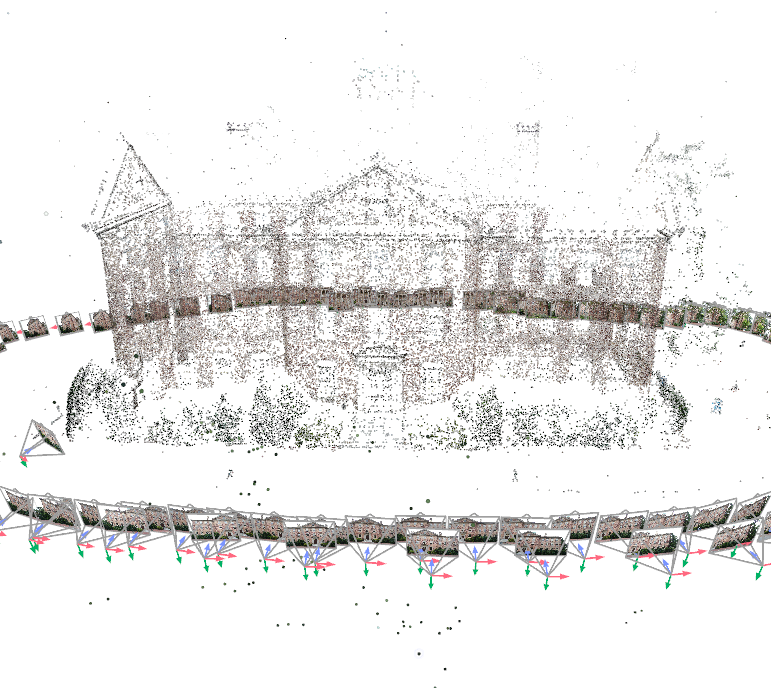
\includegraphics[width=\textwidth]{ba.png}\\
      {\scriptsize Bundle adjustment en Structure from Motion.}
    \end{column}
  \end{columns}
\end{frame}

\begin{frame}{BasaltLC - GUI: HP Reverb G2 V2 (MG*)}
  \centering
  \movie[showcontrols,loop]{\boxedimg{\linewidth}{0.88\textheight}{videos/MG.poster.jpg}}{videos/MG.webm}
\end{frame}

\begin{frame}{3- RootBA: formulación}
$\mathbf{J}_l = \mathbf{Q}\mathbf{R}$, donde $\mathbf{Q}$ es ortogonal y $\mathbf{R}$ es triangular superior, y particionando $\mathbf{Q} = [\mathbf{Q}_1\ \mathbf{Q}_2]$ de manera conforme con las filas no nulas de $\mathbf{R}$

  \begin{align}
  \left\|
  \mathbf{r}
  +
  \begin{pmatrix} \mathbf{J}_p & \mathbf{J}_l \end{pmatrix}
  \begin{pmatrix} \Delta\mathbf{x}_p \\ \Delta\mathbf{x}_l \end{pmatrix}
  \right\|^2
  &=
  \left\|
  \mathbf{Q}_1^\top\mathbf{r}
  + \mathbf{Q}_1^\top\mathbf{J}_{p}\,\Delta\mathbf{x}_p
  + \mathbf{R}_1\,\Delta\mathbf{x}_l
  \right\|^2
  +
  \left\|
  \mathbf{Q}_2^\top\mathbf{r}
  + \mathbf{Q}_2^\top\mathbf{J}_{p}\,\Delta\mathbf{x}_p
  \right\|^2.
  \end{align}

  \[
  \min_{\Delta\mathbf{x}_p}
  \left\|
  \mathbf{Q}_2^\top\mathbf{r}
  + \mathbf{Q}_2^\top\mathbf{J}_{p}\,\Delta\mathbf{x}_p
  \right\|^2,
  \]

\end{frame}


\backupend

\end{document}
